\section{بار شناختی و معیارهای اندازه‌گیری}
\label{s:CognitiveLoad}
\subsection{مقدمه}
برای شناخت حافظه می‌توان از دو دید روانشناسی شناختی، و عصب شناسی می توان استفاده کرد. در دید عصب شناسی
\LTRfootnote{Neurology}
با اجزا و المان های واقعی مغز سروکار داریم ولی در دید روان شناسی شناختی با مدل سازی سر و کار داریم که در تلاش برای شناخت و ذهن است، پس باید به خاطر داشته باشیم در روانشناسی شناختی مدل ها مفید هستند نه درست.
اتکینسون
\cite{atkinson1968human}
مدل حافظه کوتاه مدت و حافظه بلند مدت و حافظه حسی را مطرح کرد. در مدل او حافظه از سه بخش اصلی تشکیل شده است. اطلاعاتی که توسط حواس ما (بویایی، بینایی، شنوایی، لامسه و چشایی)برای مدت بسیار کوتاهی، کمتر از یک ثانیه
\cite{sperling1960information}
 ثبت می‌شوند. بسیاری از آنها حذف و بخش که مورد توجه مغز گرار می‌گیرد به حافظه کوتاه مدت منتقل می‌شود، حافظه کوتاه مدت نیز نمی‌تواند برای طولانی مدت آنها را در خود نگه دار مگر مدام آن را تکرار کند.
 \\
 اینکه چه اطلاعاتی از حافظه حسی به کوتاه مدت منتقل می‌شوند بسته به آن است که به چه چیز متوجه هستیم و منتظر دریافت آنیم.
 ویژگی مهمی که برای حافظه کوتاه مدت در نظر گرفته می‌شود مفهوم رمزگذاری
 \LTRfootnote{Encoding}
است، رمز گذاری به شکل های مختلفی انجام می‌شود.
\begin{itemize}
	\item کد معنایی 
	\LTRfootnote{Semantic Code}
	هنگامی که یک مفهوم به خاطر سپرده می‌شود.
	\item کد صوتی
	\LTRfootnote{Phenological Code}
	هنگامی که یک مفهوم در قالب آوا و صوت به خاطر سپرده می‌شود.
	\item کد حرکتی
	\LTRfootnote{Motor Code}
	هنگامی که حرکات بدن به خاطر سپرده می‌شوند.
	\item کد تصویری
	\LTRfootnote{Visual Code}
	هنگامی که یک مفهوم در قالب تصویر به خاطر سپرده می‌شود.
\end{itemize}

\begin{figure}[htbp]
	\centering
	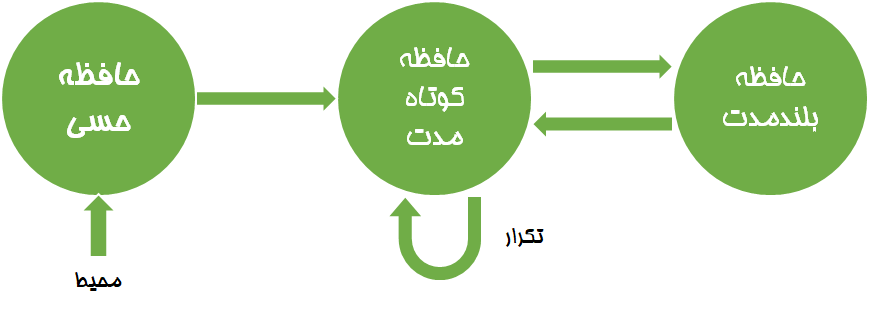
\includegraphics[width=0.7\linewidth]{figures/memory}
	\caption[تصویر مدل حافظه]{تصویر مدل ارائه شده توسط اتکینسون}
	\label{fig:memory}
\end{figure}

برای اندازه گیری ظرفیت حافظه از واحی به نام بسته اطلاعاتی
\LTRfootnote{Chunk}
استفاده می‌شود.
گفته می‌شود ظرفیت حافظه کوتاه مدت بین ۵ تا ۹ واحد اطلاعاتی است، این ظرفیت بین انسان ها متفاوت بوده جالب آنکه در یک فرد در ساعت‌های مختلف شبانه روز و حالات روحی مختلف متفاوت است.
\\
در دو دهه گذشته پیشنهاد شده است حافظه کوتاه مدت را نباید تنها محل ذخیره سازی و بازیابی اطلاعات در نظر گرفت. اگر فرض کنیم علاوه بر اینها در کوتاه مدت نیز می‌تواند با اطلاعات کار کند و آنها را پردازش کند، به مدل واقعی تر نزدیک شده‌ایم.از این رو مفهوم حافظه فعال
\LTRfootnote{Working Memory}
مطرح شده است.
\\
در این فصل، ابتدا نظریه‌ی بار شناختی معرفی و در ادامه روش‌های مختلف سنجش بارشناختی در چهار دهه گذشته بیان می‌شود.
\cite{sweller2011measuring}

\subsection{نظریه‌ی بار شناختی}
در روانشناسی شناختی، به میزان استفاده از منابع حافظه فعال گفته می‌شود. این نظریه بر مبنای ساختار شناختی انسان،‌دانش جدیدی درباره مشخصه های حافظه فعال، بلند مدت و رابطه بین این دو ارائه می‌کند.
\cite{sweller2019cognitive}
نظریه بارشناختی، سعی دارد چگونگی تاثیر بار ناشی از پردازش اطلاعات بر توانایی یادگیری اطلاعات جدید در حافظه فعال و بلند مدت را توصیف کند.
\\
پیش فرض اصلی این نظریه، محدود بودن حافظه فعال است که سبب محدودیت در توان پردازش شناختی انسان می‌شود. به طوری که تنها اطلاعات محدودی را می‌تواند در هر لحظه پردازش نماید. اگر تقاضای غیر ضروری به سیستم شناختی افزایش یابد سبب افزایش بار شناختی خواهد شد و اگر بار شناختی بیش از حد افزایش یابد سبب عدم انتقال مناسب اطلاعات و یادگیری مطلوب خواهد شد. چنین تفاضاهای غیر ضروری‌ای می‌تواند ناشی از روش‌های نامناسب آموزشی و یا پیچیدگی ذاتی محتوای تدریس شده باشد. از این رو جهت افزایش کیفیت یادگیری بهتر است بار شناختی را به نحوی مدیریت کرد که پردازش بی ارتباط با یادگیری کمینه و پردازش شناختی ذاتی یادگیری بهینه شود.
\cite{sweller2019cognitive}
\\
محدودیت حافظه کاری با توجه به اطلاعات جدید هنگام یادگیری یک تنگنا، به حساب می‌آید و تنها ۲
$\pm$
۷
عنصر اطلاعات می‌تواند در حافظه فعال نگهداری شود، این در حالی است که اگر اطلاعات نیاز به پردازش نیز داشته باشند کمتر نیز خواهد شد.
\\
به عنوان نمونه عناصر وابسته‌ای که باید باهم ترکیب شود را در یادگیری یک برنامه نوشته شده برای اجرای الگوریتم جستجوی دودویی در نظر بگیرید. یادگیری این برنامه به صورت ذاتی بسیار پیچیده تر از دستورات برنامه به صورت جداگانه است. زیرا برنامه به صورت ترکیبی از دستورات برنامه نویسی و چندین واحد اطلاعات است. در حال که دستورها را می‌توان به صورت ترتیبی از اطلاعات منفرد یاد گرفت. 
\\
بنابراین هرچه تعداد عناصر اطلاعات در تعامل با یکدیگر، در یک فعالیت بیشتر باشد، آن فعالیت سخت تر بوده و بار ذاتی بیشتری را به حافظه فعال وارد می‌کند. با این حال اطلاعاتی که پیش از این، در حافظه بلند مدت، به شکل الگوی‌های شناختی
\LTRfootnote{Cognitive schemas}
ذخیره شده است، می‌تواند بار شناختی را کاهش دهد. زیرا این الگو‌ها می‌توانند به صورت یک واحد اطلاعاتی در حافظه فعال استفاده شود، از این رو داشتین دانش پیشین در رابطه با یک فعالیت،‌ بار شناختی را کاهش می‌دهد. همچنین اگر یک فعالیت و جنبه های وابسته به آن به صورت تکراری تمرین شوند، الگو گیری شناختی خودکار شده و دیگر نیاز به پردازش کنترل شده ندارد به همین دلیل منابع بیشتری در حافظه فعال آزاد خواهند بود.
\cite{antonenko2010using}
در شکل 
\ref{fig:cognitionpatern}
الگوی شناختی دستگاه پردازش اطلاعات ذهن انسان 
در  هنگام  یادگيری  چندرسانهای  را  مشاهده می‌کنید. كلمه‌ها و  تصاویر  از  دنيای  خارج  به  صورت  ارائه 
چندرسانهای، از طریق گوش‌ها و چشم‌ها وارد حافظه حسی می‌شوند. تصاویر و متن‌های چاپی از طریق 
حافظه حسی دیداری و كلمات صحبت و دیگر صداها از طریق حافظه حسی شنيداری وارد حافظه‌ی كاری
می‌شوند. كار اصلی یادگيری چندرسانه‌ای در حافظه‌ی كاری انجام می‌شود. در این گام، الگوهای كلامی 
و تصویری (سمت راست) با استفاده از محتواهای خام وارد شده (سمت چپ) ساخته می‌شوند. دانش 
ساخته شده در حافظه‌ی كاری پس از ادغام با دانش پيشين در حافظه بلندمدت جای می‌گيرد.
\begin{figure}[htbp]
	\centering
	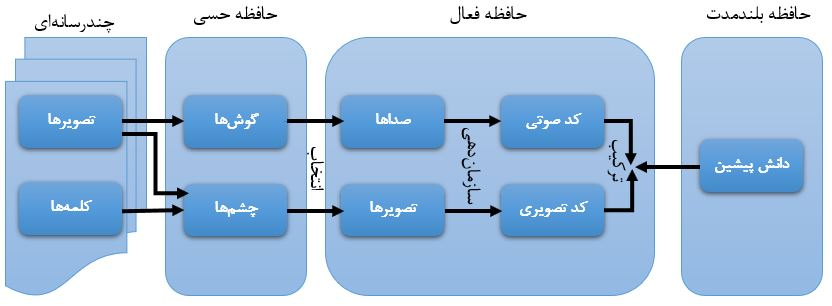
\includegraphics[width=\linewidth]{figures/cognition_patern}
	\caption[مدل الگوی شناختی یادگیری]{مدل الگوی شناختی یادگیری چند‌رسانه‌ای}
	\label{fig:cognitionpatern}
\end{figure}


\subsubsection{انواع بار شناختی}
بر اساس نظریه بارشناختی، در سه نوع بار شناختی را می‌توان مورد بررسی قرار داد: بار ذاتی
\LTRfootnote{intrinsic load}
، بار فرعی
\LTRfootnote{extraneous load}
و بار وابسته
\LTRfootnote{germane load}
.
\\
\textbf{بار ذاتی}
به پیچیدگی ذاتی محتوای در حال پردازش و نحوه تعامل عناصر اطلاعاتی گفته می‌شود که متناسب با سطح دانش پیشین یادگیرنده از موضوع اعمال می‌شود. به دلیل مشخصه های شناختی انسان، تعیین پیچیدگی اطلاعات پردازش شده دشوار است
\\
\textbf{بار فرعی}
بار ذهنی غیر ضروری است که توسط طراحی،‌ نا مناسب شناختی و ارائه‌ی نامناسب اطلاعات ایجاد می‌شود.
\\
\textbf{بار وابسته}
به عنوان منابع شناختی مورد نیاز برای دست‌کاری بار ذاتی تعریف می‌شود. این نوع بار هنگامی ایجاد می‌شود که ارائه اطلاعات برای یادگیری،‌ مفاهیم جدید و یا ماندگاری آن‌ها در ذهن طراحی شده‌باشد.
\cite{antonenko2010using}
\subsubsection{سطوح مختلف بارشناختی}
در تعریفی دیگر می‌توان گفت، بار شناختی را می‌توان اینگونه بیان نمود: باری که در طول یک فرآیند شناختی، بر حافظه فعال توسط محتوای آموزشی تحمیل می‌شود. این بار در سطوح مختلف شامل
\\
\textbf{بار لحظه‌ای}
\LTRfootnote{Instantaneous load}
نشان دهنده تغییرات بار شناختی از نخستین تا آخرین لحظه در طول یک یا چند فعالیت شناختی. این بار شناختی پایه‌ای ترین سطح سنجش بارشناختی است از این رو سایر سطح بارهای شناختی بر مبنای آن تعریف می‌شود.
\\
\textbf{بار بیشینه}
\LTRfootnote{Peak load}
،به بیشترین مقدار بار لحظه‌ای در هنگام اجرای یک فعالیت گفته می‌شود. بار بیشینه را می‌توان از طریق مقایسه بزرگی تمامی بارهای لحظه‌ای بدست آورد.
\\
\textbf{بار میانگین}
\LTRfootnote{Average load}
نمایانگر شدت بار متوسط در طول اجرای یک فعالیت و معادل مقدار میانگین بار لحظه‌ای، یا بار تجمعی در واحد زمان است.
\\
\textbf{بار تجمعی}
\LTRfootnote{Accumulated load}
مجموع مقدار باری که در طول اجرای یک فعالیت، یادگیرنده تجربه می‌کند.
\\
\textbf{بار سراسری}
\LTRfootnote{Overall load}
باری تجربی که بر پایه‌ی روند فعالیت، اعمال می‌شود. اعتقاد بر این است که بار سراسری نمایانگر دریافت شخص از تلاش ذهنی خود است.
\\
از آنجا که بار شناختی مستقیماً به مدت فعالیت بستگی دارد، هم بار میانگین و هم بار تجمعی برای تخمین اثرات طراحی آموزشی استفاده می‌شود.
\cite{antonenko2010using}
در شکل 
می‌توانید هریک از سطوح بارشناختی را مشاهده نمایید.
\begin{figure}[htbp]
	\centering
	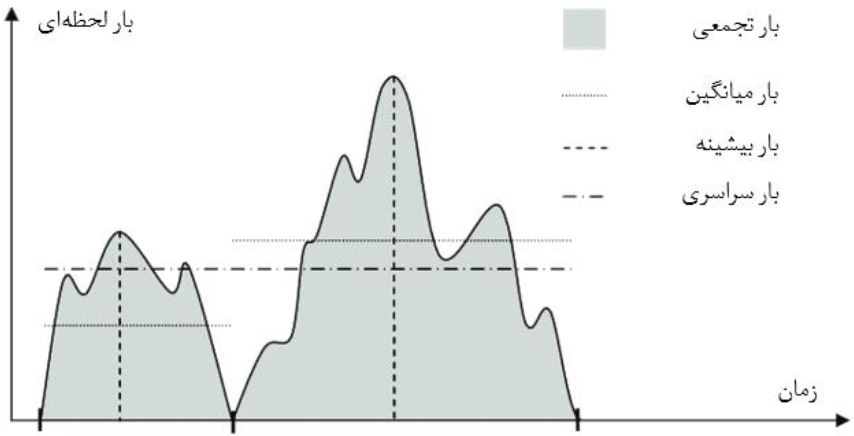
\includegraphics[width=0.7\linewidth]{figures/cl_levels}
	\caption[سطوح مختلف بار شناختی]{طرحی از سطوح مختلف بار شناختی شامل: تجمعی، میانگین، بیشینه و سراسری.}
	\label{fig:cllevels}
\end{figure}


\subsection{معیارهای سنجش بار شناختی}
هنگامی که از بار شناختی صحبت می‌کنیم یک سوال مهم راه‌های سنجش و اندازگیری آن است، این مقوله نقش جدی در پژوهش های مبتنی بر نظریه‌ي بار شناختی ایفا می‌کند از طرفی کاربردهای که در طراحی آموزش کارآمد دارد سبب اهمیت ویژه آن می‌شود.
\cite{korbach2017measurement}
\\
در ادامه روش های بیان شده در ادبیات اندازه گیری بار شناختی را مرور خواهیم کرد.

\subsubsection{کاربرد‌های سنجش بارشناختی}
علاقه به استفاده از فناوری شناختی در عمل بالینی در سالهای اخیر افزایش یافته است. کاربردهای متداول استفاده از آزمایشهای شناختی برای ارزیابی نقص در هنگام بروز اختلال‌هایی در سیستم عصبی مرکزی است. به طور نمونه چند نمنه عنوان مثال ذکر می‌کنیم:آسیب دیدگی سر، اسکیزوفرنی، سوء مصرف طولانی مدت الکل، بیماری آلزایمر و اختلال‌های مرتبط با آن، هستند.
\\
علاوه بر این ، از آنجا که مهارت های شناختی با زندگی روزمره و فعالیت های اجتماعی همراه است،ارزیابی شناختی می تواند در غربالگری  و پایش بیماران ترخیص‌شده و در ساخت راهکارهای توانبخشی فردی سودمند باشد.
\\
از آنجا که بار شناختی در نتیجه حافظه کاری محدود در حین کار ایجاد می شود ، اندازه گیری بار شناختی بر روی بیماران در آزمایش‌های شناختی می تواند بینش هایی را برای معالجه بیمار ارائه دهد.
به عنوان مثال، بار شناختی زیاد و مدت زمان محرک کوتاه برای ایجاد تمایز برای بیماران اسکیزوفرنی پیدا شد.
سایر کاربردها شامل کاهش خطاهای پزشکی به دلیل بار زیاد حافظه پزشکان در اورژانس است.
مطالعات نشان داده است که وقفه ها (باعث از بین رفتن اطلاعات) و چندکار را هم‌زمان انجام دادن باعث افزایش بار شناختی می شود که به خطاهای پزشکی کمک می کند.
راه حل های ارائه شده شامل استفاده از ابزارهای الکترونیکی برای پشتیبانی از روند به صورت تطبیقی در محل کار و ارائه آموزش های مؤثر جهت کاهش بار شناختی در محل کار است.
تمرکز دیگر بر ارزیابی سیستم های اطلاعات بالینی است. رویکردها مبتنی بر مهندسی کردن قابلیت‌ها و موارد استفاده و   تجزیه و تحلیل وظیفه شناختی است تا اطمینان حاصل شود که  در حالی که کاربران در حال انجام وظایف هستند کمترین بار شناختی در استفاده از چنین سیستم‌هایی مصرف شود.
\subsubsection{معیار های غیرمستقیم سنجش بارشناختی}
در نخستین روزهای ارائه نظریه بارشناختی، بار شناختی به صورت مستقیم اندازه گیری نمی‌شد یکی از اولین روش‌ها بر اساس نتایج آزمایش‌ها،‌ ارتباط میان بار شناختی و حل مسئله بود، از این رو چندین روش برای ارزیابی غیر مستقیم بار شناختی مورد استفاده قرار گرفت.
\cite{sweller2011measuring}
\paragraph{الگوهای محاسباتی}
نخستین پژوهش‌ها تمرکز خود را بر روی ناکارآمدی حل مسئله به عنوان راهبرد یادگیری تمرکز کرده‌ بودند. این گونه فرض می‌شد که کاوش بر روی مسئله سطح بالا منجر به بار بیشتر بر روی حافظه فعال و تلاش برای حل مسئله سطح پایین منجر به بار حافظه فعال کمتر خواهد شد.
\cite{sweller2011measuring}
\\
در یک مجموعه از آزمایشها ،سویلر و همکاران نشان دادند كه راهبرد یادگيری كه شامل جستجوی
قابل توجه در حل یک مسئله است، منجر به یادگيری پایينتری نسبت به مسئله‌ای كه نيازمند جستجوی
بالاتری داشت،  شده  است. سویلر  استدلال  كرد  كه  برخی از  راهبردها منجر  به  این شد  كه  جستجوی
بيشتری برای حل  مسئله  نياز باشد  و  همين امر  موجب  افزایش بار شناختی  فرعی شد.  در  مقابل 
فرآیندهایی كه جستجو برای حل مسئله را كم می‌كنند، باعث كاهش بار شناختی شدند. پشتيبانیهای
نظری كه نشان می‌دهند جستجو برای حل مسئله، بار شناختی را افزایش می‌دهد، از طریق الگوهای 
محاسباتی نشان  داده  شده  است. سویلر  متوجه  شد  كه برای ساخت  الگوهایی جهت  مقایسهی حالت 
جستجوی زیاد با حالت جستجوی كم، باید برای الگوهای نيازمند جستجوی زیاد، الگوهای پيچيدهتری
طراحی كرد تا نياز باشد كه اطلاعات متناظر بيشتری را در حافظهی كاری نگهداری شود.
\cite{tarmizi1988guidance}
شواهد غیر مستقیم الگوهای محاسباتی، سبب استفاده محدود از آنها شده است. با این در نظریه بار شناختی الگوهای محاسباتی اولین تلاش برای ارائه شواهد بودند و عامل مهمی در ریشه‌های نظریه‌ی بار شناختی محسوب می‌شوند.
\cite{sweller2011measuring}
\paragraph{کارایی در طول یادگیری}
در مطالعه‌های نخستین اندازه‌گیری بار شناختی، راه هایی برای اندازه گیری بارشناختی در طول فرایند یادگیری دیده می‌شود.
\cite{sweller2011measuring}
روش پیشنهاد شده توسط چندلر و سویلر زمان آموزش را به عنوان ملاکی برای اندازه بار شناختی مطرح کرد. این دو محقق بر این باور بودند که اگر دانش آموزش در یک فرایند یادگیری که بار شناختی آن به مرور افزایش پیدا می‌کند شرکت کند، این افزایش بار شناختی، بر عملکردش در هنگام یادگیری نیز تاثیر می‌گذارد. نتیجه آن را می‌توان در هر دو عملکرد پایانی و طول فرایند یادگیری مشاهده نمود.
\cite{chandler1991cognitive}
شواهدی دیگر نشان دادند با افزایش بارشناختی، نرخ خطا بالا رفته که سبب کاهش دقت و افزایش زمان یادگیری می‌‌شود.

\paragraph{خطاهای نمایه بین مسئله‌ها}
نرخ خطا نیز برای اندازه گیری بار شناختی و به طور خاص شناسایی تفاوت های شناختی مسئله ها مورد بررسی قرار گرفت.
آیریس و سویلر مشاهده کردند، دانش‌آموزان در حل مسائل هندسه در برخی مرحله ها به دلیل دشوار شدن مسئله و در نتیجه آن درگیر و پر شدن حالظه فعال دچار خطا می‌شوند.
\cite{ayres1990locus}
در دسته‌ای دیگر از مطالعه‌های آیریس نشان داد، در حین یک تکلیف ریاضی که نیازمند محاسبه‌های پشت سر هم بود، نرخ خطا متفاوت است. نرخ خطای بالا در دو حالت رخ می‌داد: اول آنکه شدت نیاز به تصمیم گیری افزایش پیدا کند و دوم آنکه تعداد متغیر های مورد نیاز افزایش پیدا کند.
\cite{ayres2001systematic}
این نقد وجود دارد که این دو مطالعه بر روی حل مسئله های ریاضی بررسی شده است و نه فرآیند یادگیری، با این حال با استفاده از شواهد نشان دادند، نرخ خطا با نیازمندی های حافظه فعال در ارتباط است.
\subsubsection{معیارهای خودانگارانه سنجش بارشناختی}
در گذشته،‌ برای پیش‌بینی کارایی و اثر بخشی آموزش از از ملاحظه‌های نظری استفاده می‌شد که عمدتا شامل معیار های غیر مستقیم همانند زمان و نرخ خطا در یادگیری بودند. با توسعه نظریه بار شناختی و اثر‌های آموزشی نیاز به معیار های مستقیم بیشتری برای بار شناختی آشکار شد. پاس با معرفی روش اندازه گیری خودانگارانه بار شناختی دست آورد مهمی به بار آورد.
\paragraph{معیارهای خودانگارانه برای سنجش تلاش ذهنی}
پاس بیان کرد دانش آموزان خود می‌توانند بر اساس تلاش ذهنی صرف شده شان در طول فرآیند یادگیری و آزمون تلاش ذهنی خود را اندازه گیری کنند، و این امتیاز می‌تواند شاخصی برای بار شناختی در نظر گرفته شود. این برداشت بر اساس ابزاری بود که پیش از این خود پاس آن را توسعه داده بود.
\cite{paas1992training}
تلاش ذهنی این گونه تعریف می‌شود:
\\
\textit{تلاش ذهنی }
جنبه‌ای از بار شناختی که به ظرفیت شناختی اختصاص داده شده به تقاظای موردنیاز تکلیف،‌اشاره می‌کند و می تواند بازتابی برای بار شناختی واقعی در نظر گرفته شود.

\paragraph{مقیاس ۹ نقطه‌ای لیکرت}
\LTRfootnote{9-point Likert Scale}
این مقیاس در بازه عدد یک تا نه قرار دارد، یک معادل خیلی خیلی کم و نه معادل خیلی خیلی زیاد برای تلاش ذهنی است، از این مقیاس می‌توان در حین یادگیری و یا آزمون استفاده نمود. در مقایسه با روش های آموزشی که در آنها سعی در افزایش و یا کاهش بار شناختی می‌شد، پاس انطباقی بین امتیازدهی شخصی تلاش ذهنی و عملکرد آزمون پیدا کرد. به دو گروه از دانش آموزان دو دسته سوال متفاوت داده شد دسته اول سوال‌های سخت و پیچیده‌تر و دسته دوم سوال‌های ساده تر، مشاهده شد که به گروهی که سوال‌های سخت‌تر داده شده بود، خود تلاش ذهنی بیشتری گزارش کرده بودند و از طرفی عملکرد آنها نسبت به دسته دیگر کمتر بود.
\cite{paas1992training}
\\
در آزمایشی دیگر از پاس و ون‌مرینبور با جمع‌آوری و تجزیه و تحلیل طیفی ضربان قلب به بررسی معیار های فیزیولوژیکی پرداختند. معیار های فیزیولوژیکی تنها قادر به تشخیص تفاوت بین دوره‌های فعال و غیر فعال ذهنی بود، و نمی تواست میان گروه‌های رفتاری تمایزی پیدا کند. از طرفی دیگر امتیازدهی های خود انگارانه، بسیار حساس‌تر و موثر تر بار شناختی را می‌سنجیدند، مقیاس ۹ نقطه‌ای لیکرت نیز بسیار قابل اعتماد بود.
\paragraph{معیار خودانگارانه برای سنجش دشواری}
سایر پژوهشگران با مشاهده موفقیت معیار‌های خودانگارانه، این مقیاس خود انگارانه را به عنوان معیاری برای اندازه گیری بار شناختی پذیرفتند. به عنوان مثال در یک مجموعه از آزمایش ها، مشاهده شده است که میزان دشواری با اندازه گیری های خود انگارانه به طرز قابل توجی تطابق دارد.
\cite{marcus1996understanding}
می توان گفت سادگی و حساس بودن مناسب مقیاس امتیازدهی این روش را مورد توجه پژوهشگران قرار داده است.
\paragraph{گوناگونی در امتیازدهی های خودانگارانه}
ون‌گوک و پاس با استفاده از پژوهش هایی بیان کردند که کلمه تلاش ذهنی و دشواری ذهنی در پرسشنامه خودانگارانه ممکن است نتایج متفاوتی را در بر داشته باشد.
باید دقت کنیم پرسیدن تلاش ذهنی از یک دانش آموز و میزان تلاش صرف شده توسط وی متفاوت است، البته اغلب این دو معیار با یکدیگر همبستگی نیز دارند، گاه نیز با یکدیگر تطابق ندارند. به طور نمونه، مسئله های بسیار دشوار ممکن است از دید بعضی از دانش آموزان به نحوی باشد که قادر به پاسخگویی آن نباشند، و در نتیجه آن هیچگونه تلاشی را انجام ندهند.
\cite{van2008instructional}
\\
پاس و ون‌مرینبور اندازه گیری تلاش ذهنی را پس از مرحله ی یادگیری و حل مسئله، ثبت کردند. به علاوه بسیار از پژوهشگران داده ها را بعد از اتمام دوره‌ی آموزش جمع آوری می‌کنند. دو راهبرد، لزوما، قابل مقایسه نیستند و ممکن است نتایج مختلفی به دست آورند. بعضی از این اختلاف‌ها در هنگام بحث در مورد اقدامات کارآیی در نظر گرفته نمی‌شود.
\cite{paas1994measurement}
\paragraph{پایداری در معیارهای خود انگارانه}
روش های اندازه گیری خودانگارنه شامل تلاش ذهنی و یا دشواری ذهنی در عین گوناگونی و تفاوت بسیار امید بخش بوده‌اند، از این جهت که به طرز شگفت انگیری با داده های عملکردی پیش‌بینی شده توسط نظریه‌ی بار شناختی کمترین تناقض، سازگار و مطابق بوده است. با این حال در برخی مطالعه‌ها، تفاوت های قابل ملاحظه‌ای میان اندازه گیری های خود انگارانه و آزمون عملکرد مشاهده شده است.
\cite{sweller2011measuring}
\\
همچنين مطالعه‌‌هایی وجود دارد كه در آن تفاوت بار شناختی بر اساس معيارهای خودانگارانه وجود دارد 
اما هيچ اثری از گروههای رفتاری بر روی آزمونهای عملکرد وجود ندارد. كاليگا، چندلر و سویلر در هر یک
از  سه آزمایش نتایج متفاوتی را  به  دست  آوردند:  تفاوت  در  بار  شناختی بدون  اثر  آزمون؛  تفاوت  در  بار 
شناختی و اثر آزمون متناظر؛ بدون تفاوت بار شناختی اما با اثر آزمون. این امکان وجود دارد كه تحت 
شرایط و مواد آموزشی خاصی، هيچ گونه تطابقی رخ ندهد. البته با در نظر گرفتن هرگونه اثر آماری تعيين
شده، ناگزیر، تطابق با شکست روبرو خواهد شد. همبستگی بين مقياس امتيازدهی خودانگارانه و آزمون
عملکرد نمی‌تواند كامل باشد. با وجود ناسازگاری گاه به گاه، معيارهای خودانگارانه تاكنون نفوذ عميقی
داشته و یک ابزار مفيد برای ارائهی شواهد در پشتيبانی از نظریهی بار شناختی فراهم آورده است.
\cite{kalyuga2004redundant}
\subsubsection{معیار های کارآیی}
پاس و ون‌مرینبور مقتقد بودند در نظر گرفتن هزینه‌های شناختی یادگیری مهم است، از این رو بر اساس مقیاس خود انگارانه، یک معیار کارایی که تلاش ذهنی و شاخص‌های عملکرد را در می‌گرفت توسعه دادند. نکته مهم این است که با وجود اینکه ممکن است دو روش آموزش متفاوت از یکدگیر باشند و نتایج یادگیری مشابهی داشته باشند، اما تلاش برای رسیدن به این سطوح عملکرد نیز مهم است. اگر دو راهبرد آموزشی متفاوت منجبر به عملکرد یکسان شوند، راهبردی کارآمدتر است که منابع شناختی کمتری صرف آن شده باشد، کارایی (E) را میتوان از رابطه زیر محاسبه نمود:
\begin{equation}\label{eq:efficiency}
E = \frac{(Z_{Ptest}-Z_{PEtest})}{\sqrt{2}}
\end{equation}
همان گونه که در رابطه 
\eqref{eq:efficiency}
مشاهده می‌کنید،
$ Z_{Ptest} $
بازنمایی نرمال شده با میانگین صفر
\LTRfootnote{Z-score normalization}
نمره‌های آزمون و 
$ Z_{Etest} $
نرمال شده با میانگین صفر نمره‌های تلاش ذهنی است که پس از دوره‌ی آزمون جمع آوری شده‌اند. این رابطه بر مبنای محاسبه‌ی فاصله عمود از یک نطقه به یک خط راست تعریف شده است. همان طور که در شکل 
\ref{fig:efficiency}
نشان داده شده‌است،
z-score
اگر تلاش و کارآیی یکسان باشد مقدار E صفر خواهد بود و تمامی نقاطی که روی این خط قرار دارند نیز معادل با 
$ E = 0 $
هستند، از طرفی تمامی نقاطی که بالای آن قرار می‌گیرند کارایی آنها مثبت بوده و یادگیری در آن حالت موثر و کارا است 
$ (E > 0) $
و بلعکس تمامی نقاط زیر خط کارآیی آنها منفی است و در نتیجه یادگیری در این حالت ناکارآمد و غیر مفید است.
$ (E < 0) $
.
\cite{paas1993efficiency}
همچنین پاس و همکاران نشان دادند کارایی بالا در آموزش از عملکرد بالا در آزمون و تلاش کم حاصل می‌شود(ناحیه حاشور خورده در نمودار) و کارآیی آموزشی کم نتیجه عملکرد ضعیف در و تلاش ذهنی بالا است(ناحیه نقطه‌ای در نمودار).
\cite{paas2003cognitive}
\\

\begin{figure}[htbp]
	\centering
	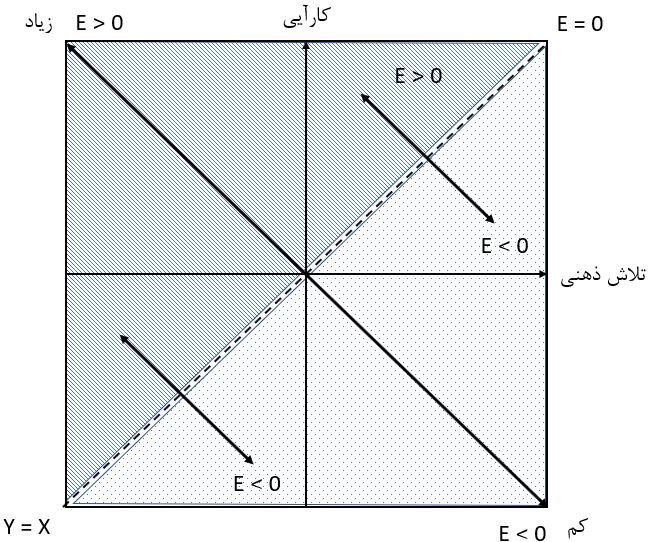
\includegraphics[width=0.7\linewidth]{figures/efficiency}
	\caption[بازنمایی گرافیکی کارآیی]{محور افقی نشان دهنده تلاش ذهنی و محور عمودی کارآیی خواهد بود، طبق شکل نواحی حاشور خورده دارای کارایی مثبت و نواحی نقطه‌ای دارای کارآیی منفی هستند.}
	\label{fig:efficiency}
\end{figure}

در یک بررسی دیگر توسط پاس و ون‌گوک از سال ۱۹۹۳ تا ۲۰۰۷ که بیش از ۳۰ مورد پژوهش در رابطه با نظریه‌ی بار شناختی را شامل می شد که از معیار کارآیی استفاده کرده بودند. با این حال همان طور که پاس و ونگوک اشاره کرده بودند تفاوت هایی بین روش امتیاز دهی ذهنی وجود داشت باعث ایجاد تفاوت‌هایی که در روش امتیاز دهی ذهنی وجود داشت باعث ایجاد تفاوت هایی در کارآیی شده است. زیرا كارآیی طبق  فرمول  به 
اندازهگيریهای ذهنی بستگی دارد. آنها اظهار داشتند كه رویکردهای گوناگون، انواع مختلف كارآیی ر ا 
می‌سنجد.  استفاده  از  امتياز های ذهنی  جمع آوری شده  پس از  آزمون،  عواقب  یادگيری ساخت
ساختارهای شناختی نظير الگوهای ذهنی را اندازهگيری می‌كند، درحالیكه اندازهگيریهای بعدی نشان
دهندهی كارآیی آموزش است.
\cite{van2008instructional}
\\
كارآیی یادگيری می‌تواند شاخص خوبی برای طراحی و خودكارسازی باشد. اگر دانش آموزان الگوهای
جدیدی به دست آورند و بتوانند با استفاده از آنها با تلاش كمتری یاد بگيرند، آن الگو قوی به حساب
می‌آید حتی اگر طراحی آموزشی بيشتری نياز باشد. با این وجود، بازدهی آموزشی نقش مهمی دارد، زیرا
نشان می‌دهد كه فرآیند یادگيری به چه شکل كارآمد است. دانستن ميزان سختی یا آسانی در طراحی
آموزشی، نقش مهمی در نظریهی بار شناختی دارد. با وجود این تفاوت در رویکردها، هر دو محاسبه كار آیی
آموزش و عملکرد در یادگيری اطلاعات در یک آزمون مهم هستند و می‌توانند اطلاعات حياتی مربوط به 
طراحی آموزشی را فراهم كنند.
\cite{sweller2011measuring}
\paragraph{مسائل مهم محاسبه‌ی کارآیی}
با وجود استفاده در مقياس وسيع، هافمن و شارو برخی از نگرانیهای مربوط به محاسبه كارآیی
آموزشی را شناسایی كردند. در بررسی كارآیی، آنها مدل اصلی پاس و ونمرینبور را به عنوان یک الگوی
انحراف
\LTRfootnote{Deviation model} 
دسته بندی كردهاند، زیرا بر اساس اختلاف بين نمر ههای عملکرد و تلاش استاندارد شده، 
محاسبه می‌شود. آنها استدلال كردند كه تفسير معنای تفریق دو متغير كه متفاوت از یکدیگر هستند ،
دشوار است. آنها این مثال را مطرح كردند كه مشابه این است كه هوش و وزن فرد را كه به صورت z-score
درآمدهاند را از هم كم كنيم. بنابراین تفسير نتيجهی نمرهی به دست آمده مشکل است.
\LTRfootnote{text}
\cite{hoffman2010conceptions}
آنها همچنين اشاره كردند كه اندازهگيری كارآیی تنها میتواند بر اساس دادههای گروهی باشد و در
نتيجه نمی‌تواند برای مقایسهی كارآیی فرد استفاده شود. از سوی دیگر آنها پيشنهاد كردند كه تفاوتهای
یافت شده در رفتار كلی مقایسه شود. بيشتر مطالعه‌های انجام شده در چارچوب نظریه‌ی بار شناختی به طور
كلی بر روی تفاوتهای گروهی تمركز می‌كنند، بنابراین مقایسه‌های فردی مسئله‌ای نيست. هافمن و شارو به عنوان جایگزینی برای مدل انحراف، مزایای دو روش دیگر را توصيف كردند: الگوی احتمال ،
\LTRfootnote{Likelihood model}
بر اساس 
نسبت عملکرد و امتيازدهی و الگوی احتمال شرطی ،
\LTRfootnote{Conditional likelihood model}
بر اساس نسبت احتمالها.
\cite{hoffman2010conceptions}
هافمن و شارو، مدل انحراف را  ضعيف نمی‌دانند بلکه مدعی هستند كه الگوهای مختلف با اهداف 
تحقيق مختلف ،متفاوت هستند. با این وجود، بر اساس تجزیه و تحليل هافمن و شارو محاسبهی نسبت 
عملکرد  و  امتيازدهی خودانگارانه (الگوی احتمال) بسيار ساده  است  و  می‌توانند برای تعيين اندازه‌ی
كارآیی فردی مورد استفاده قرار گيرند. این اندازهگيری‌های خودانگارانه می‌توانند به راحتی تركيب شود تا 
كارآیی گروهی را كه برای مقایسه‌ی رفتارهای كلی ضروری است فراهم كنند. انتظار می‌رود پژوهش‌های
آتی برای محاسبهی كارآیی، بيشتر از الگوهای احتمالاتی استفاده كنند.
\cite{hoffman2010conceptions}
\subsubsection{سنجش بارشناختی از طریق یک کار ثانویه}
معيارهای ذهنی كه  در  بالا  شرح  داده  شدند،  شایعترین ابزار  مورد استفاده  برای اندازهگيری بار 
شناختی بودند. با این حال، روش سنتی برای ارزیابی بار حافظهی كاری استفاده از كار ثانویه است كه با 
كار اصلی
\LTRfootnote{Primary task}
تركيب می‌شود (روش دوگانه) .یک كار ثانویه، مستلزم این است كه یادگيرنده علاوه بر كار 
اصلی یا حل مسئله، با فعاليت شناختی دیگری كه به كار اصلی اضافه می‌شود، درگير شود. برای مثال، در
حالی كه فرد در حال یادگيری چگونگی حل یک مجموعه مسائل ریاضی است، از وی خواسته می‌شود تا به 
نحو مشخصی به یک صدای خاص به عنوان یک فعاليت ثانویه پاسخ دهد. اگر كار اصلی بار شناختی
سنگينی را تحميل كند، عملکرد در كار ثانویه بدتر می‌شود. در مقابل، بار شناختی كمتر در كار اصلی
می‌تواند عملکرد بهبود یافته در كار ثانویه را افزایش دهد.
\cite{sweller1988cognitive}
\\
معمولا، كار ثانویه كاملا متفاوت با كار اصلی و نياز به منابع حافظه كمتر نسبت به كار اصلی دارد؛ با این
حال،  سویلر یک جایگزین برای این قالب ایجاد كرد.  سویلر معتقد  است  كه  درخواست  كردن  از  دانش
آموزان در حل مسئله از طریق یادگيری شامل دو فرآیند است:
\begin{enumerate}
	\item حل مسئله، كار اصلی
	\item یادگيری از 
	طریق تجربه، كار ثانویه.
\end{enumerate}
به عبارت دیگر، زمانی كه فراگيران در حال حل مسئله به عنوان وظيفهی اصلی
هستند، ممکن است این درگيری بر عملکرد كار ثانویه تأثير بگذارد. مشکل پيچيدهتر این است كه كمتر در 
مورد كار ثانویه یاد بگيرند. شواهد تجربی بر اساس یک كار خاص ثانویه كه شامل یادآوری دادهها و راه حل 
یک مشکل  پيشين است،  این استدلال  را  پشتيبانی  می‌كند.  فرآیندهای آموزشی در  جهت  كاهش  بار شناختی مرتبط با حل مسئلهای كه اطلاعاتی كه نياز به یادآوری برای حل مسئلهی قبلی دارد حركت 
می‌كند.
\cite{sweller1988cognitive}
\\
در یک استفاده  سنتی از  یک كار  ثانویه، ماركوس  و  همکاران  تعامل  با  عناصر  ارائهی آموزشی را 
موردبررسی قرار دادند و به طور خاص بررسی كردند كه یک نمودار چگونه تعامل با عناصر را  نسبت به 
حالتی كه فقط متن نمایش داده می‌شود، كم می‌كند. در این مطالعه، دو نوع كار ثانویه مورداستفاده قرار 
گرفت كه در هر دو، كار اصلی یکسان بود. در یک آزمایش، كار ثانویه این بود كه صدای بوق را كه به صورت 
تصادفی در طول یادگيری پخش می‌شود، تشخيص دهند. یادگيرندگان باید به محض شنيدن صدا، یک
پدال پایی را  فشار می‌دادند .زمان پاسخ
 \LTRfootnote{Response time}
به عنوان معياری برای اندازهگيری بار شناختی اعمال شده 
توسط كار اصلی، مورداستفاده قرار گرفت. در آزمایش دوم، كار ثانویه، یادآوری اعداد دو رقمی بود كه در 
حين كار اصلی به نمایش درمی‌آمدند. در این مورد، دقت یادآوری اعداد در كار ثانویه، به عنوان معياری
برای اندازهگيری بار شناختی استفاده شد. برای هر دو نوع كار ثانویه، نتایج قابل توجهی در تطابق با نتایج
یادگيری به دست آمد. استفاده از نمودارها و محتوای تعاملی كه منجر به نتایج بهتر، یادگيری و عملکرد
قویتر در وظایف ثانویه شد. از این رو در این پژوهش، توصيف بار شناختی مورد پشتيبانی قرار گرفت.
\cite{marcus1996understanding}
چندلر و سویلر نيز از یک روش دوگانه استفاده كردند تا نشان دهند كه كار ثانویه، كه یادآوری یک نشانه
بود، تحت تأثير قسمت آموزش قرار گرفته است. برای كار ثانویه، دو نشانهی جداگانه با صدای بوق  8ثانيه
بر روی صفحه نمایش كامپيوتر نمایش داده شد. یادگيرنده باید نشانهی اول را، در حالی كه نشانهی دوم را 
به خاطر می‌سپارد، به یاد آورد. نتایج نشان داد كه راهبرد آموزشی كه بار شناختی كمتری اعمال كند ،
دارای نمرههای بالاتری در كار ثانویه است. علاوه بر این، تفاوتهای قابل توجهی تنها برای راهبردهای
آموزشی و اقدام‌‌های ثانویه یافت شد، زمانی كه محتوای یادگيری دارای تعامل بالا با عناصر بودند. برای
محتوایی كه كمتر در تعامل با عناصر بودند، منابع حافظهی كاری بيشتری برای درگيری با كار ثانویه در 
دسترس بود، در نتيجه نتایج بهتری در آن به دست آمد و كمتر تحت تأثير قرار گرفت.
\cite{chandler1996cognitive}
در كارهای حل 
مسئله، در مقایسه با سایر وظایف، هالفورد، ميبری و باین
\cite{halford1986capacity}
و آیریس
\cite{ayres2001systematic}
از یک كار ثانویه استفاده
كردند تا نشان دهند كه تعامل بالا با عناصر، با بار حافظهی كاری بالا مطابق است.
\\
برونکن، اشتاینباخر، پلس و لوتنر از یادگيرندگان خواستند كه تغيير رنگ نشانههایی را كه در بالا ی
ارائه‌ی اصلی نمایش داده می‌شد ،رصد كنند. هنگامی كه رنگ تغيير كرد، یادگيرنده باید كليدی را كه روی
صفحه كليد مشخص شده است، فشار دهد. زمان پاسخ در این پژوهش، برای اندازهگيری بار شناختی استفاده شد. نتایج نشان دادند كه برای ارائههایی كه خوب طراحی شده بودند، بهترین عملکرد حاصل شد 
و دوباره از نظریهی بار شناختی پشتيبانی گردید.
\cite{brunken2004assessment}
\\
در پژوهش قبلی، كار ثانویه دیداری بود .در مطالعهی بعدی، برونکن ،پلس و لوتنر كار ثانویهی شنيداری
را موردبررسی قرار دادند. با استفاده از این استدلال كه محتوای شنيداری و دیداری در زیرسيستمهای
مختلف حافظه‌ی كاری پردازش می‌شوند، برونکن و همکاران معتقدند كه حالتهای مختلف (دیداری و 
شنيداری) كارهای ثانویه باعث بروز بار شناختی گوناگون در كانالهای مختلف حافظهی كاری خواهد شد.
به طور  خاص،  یک كار  ثانویه شنوایی باعث ایجاد تفاوتهای بار  شناختی در  كانال  شنوایی خواهد 
شد.
\cite{brunken2004assessment}
این فرض با استفاده از همان محتوای آموزشی كه برونکن و همکاران استفاده كردند انجام شد، 
با این تفاوت كه به جای رصد  كردن تغيير رنگ نشانهها، از صدای بوق كه به صورت تصادفی در طول 
آزمایش پخش  می‌شد، استفاده  كردند.  این بار  نيز از  زمان  پاسخ  به عنوان  معياری برای بار شناختی
استفاده گردید. همان طور كه پيشبينی می‌شد، كار ثانویهی شنيداری در مقایسه با كار ثانویهی دیداری،
موجب افزایش بار شناختی بيشتری در كانال شنوایی شد.
\cite{brunken2002assessment}
این دو مطالعه نشان دادند كه چگونگی
كار ثانویه عامل مهمی است كه باید در نظر گرفته شود.
\\
ون‌گرون، پاس، ونمرینبور و اشميت یک كار ثانویهی شنيداری-دیداری را موردبررسی قرار دادند. در 
این مطالعه، در  كار  ثانویه از  یادگيرندگان درخواست  شد  كه  روشنایی دكمهی یک نوع وسيلهی  پخش 
موسيقی
\LTRfootnote{Jukebox}
 را  كه  روبه‌روی محتوای آموزشی نشان داده  می‌شد، رصد  كنند. در این مطالعه  كار ثانویه‌ی
شنيداری-دیداری با كار ثانویهی تنها دیداری و تأثير سن موردبررسی قرار گرفت. نتایج یادگيری نشان داد 
كه افراد جوان بهتر از افراد مسن عمل كردند ولی اثری برای كيفيت محتوای آموزشی پيدا نشد. كار ثانویه،
این نتيجه را برگرداند: یادگيرندگان جوان، زمان پاسخ كمتری را نسبت به یادگيرندگان مسن داشتند. به
علاوه، اندازهگيری فردی بار شناختی نيز جمع آوری شد كه تفاوتهای ميان سن و كيفيت را نشان می‌داد .
جالب اینکه، حتی اگر هيچ اثری ناشی از كيفيت بر عملکرد آزمون وجود نداشت، اندازه‌گيری فردی،
ارائهی دوگانه  را  بهتر از  حالت ارائه‌ی واحد،  ارزیابی كرد.  این آزمایش نشان داد  كه  ارزیابی فردی، بار
شناختی را بهتر از كار ثانویه اندازه‌گيری می‌كند.
\cite{van2006modality}
\\
پژوهشها در حوزه نظریهی بار شناختی، كمتر از كار ثانویه نسبت به ارزیابی فردی به عنوان معياری
برای بار شناختی استفاده كردهاند. شاید سهولت استفاده دليل اصلی این تفاوت در استفاده از این دو 
روش باشد. ارزیابی فردی می‌تواند به سرعت و سادگی مورداستفاده قرار گيرد. این معيار را می‌توان برای
یک شخص یا تعدادی دانش آموز در یک كلاس، بدون امکانات خاصی به كار برد. در مقابل، كار ثانویه به برنامه ریزی بيشتری نياز دارد  و  بسته  به  طبيعت كار  ثانویه ممکن  است امکانات  خاصی نياز داشته 
باشد.
\cite{sweller2011measuring}
\\
با این وجود، مزیتهایی نيز در استفاده  از  كار ثانویه وجود  دار د.  مزیت اصلی این است كه  امکان
اندازهگيری بار شناختی پيوسته در طول یک كار فراهم است، در حالی كه ارزیابی فردی، بار سراسری
شناختی را پس از پایان كار اندازه‌گيری می‌كند.
\cite{sweller2011measuring}
\\
تاكنون اندازه‌گيری كارآیی با استفاده از كار ثانویه محاسبه نشده است. هيچ دليلی برای محاسبه نشدن
آنها وجود ندارد. تمامی معيارهای كارآیی كه توسط هافمن و شارو
\cite{hoffman2010conceptions}
بررسی شد می‌توانند به سادگی
توسط كار ثانویه به عنوان یک ارزیابی فردی محاسبه شوند، كه یک ارزش گذاری جدید برای بار شناختی
ایجاد می‌كند.
\subsubsection{سنجش فیزیولوژیکی بار شناختی}
% Chen, S., & Epps, J. (2013). Automatic classification of eye activity for cognitive load measurement with emotion interference.
چِن و اِپس
\cite{Chen2013}
با طبقه بندی داده‌هایی که توسط دستگاه ردیاب چشمی از کاربر گرفته‌ می‌شود توانستند معیار خوبی برای اندازه‌گیری بارشناختی به صورت هم‌زمان به‌دست آورند. از جمله ویژگی های اندازه گیری شده می‌توان به قطر‌ مردمک چشم، پلک زدن و حرکت‌های چشم اشاره کرد. آزمایش آن‌ها محاسبه‌‌های ریاضی و نشان دادن عکس به کاربر بود.
% pass

پاس و و نمرینبور یک معيار فردی را با تحليل نرخ ضربان قلب مقایسه كردند و نتيجه این بود كه معيار
فردی دارای پتانسيل بالاتری است.  تعداد  كمی از  مطالعات  فيزیولوژیکی پس از آن  توسط پژوهشگران 
نظریه‌ی بار شناختی در دهه‌ی بعد انجام شد. با این حال اخيرا، دوباره علاقه به این اقدامات ظهور كرده 
است.  واكنش  مردمکهای چشم
\LTRfootnote{Pupillary response}
به فعاليتهای شناختی، راهبرد دیگری بود  كه  امتحان شد.
\cite{paas1994variability}
ونگرون،  پاس، ونمرینبور و  اشميت با اشاره به  كار كاهنمن و بيتی
\cite{kahneman1966pupil}
،استدلال كردند كه  اندازه‌ی
مردمک  می‌تواند به  بار  حافظه‌ی كاری مربوط  باشد.  با  استفاده  از یک مجموعه تکاليف كه  نياز به  بار 
حافظهی مختلفی داشتند،  پيشنهاد كردند  كه  اندازهی مردمک  چشم،  با  افزایش بار حافظه، بيشتر
می‌شود. با این وجود یکی از محدودیت این معيار، سن فرد است زیرا با افزایش سن، همبستگی این معيار
با بارشناختی كم می‌شود و پاسخ قابل اعتمادی به دست نمی‌آید.
\cite{van2004memory}
پژوهشگران برای اندازهگيری بار شناختی از روشهایی مانند تصویرسازی تشدید مغناطيسی كاركردی
(اف‌ام‌آرآی)
\LTRfootnote{Functional Magnetic Resonance Imaging(FMRI)}
و الکتروانسفالوگرافی (ای‌ای‌جی) نيز استفاده  كرده‌اند.  این علاقه  همزمان  با  توسعه‌ی
فناوری‌های پيچيده‌تر بود.  شواهد نشان می‌دهد كه  روشهای فيزیولوژیکی می‌توانند شایستگی قابل
توجهی داشته باشد.
\cite{sweller2011measuring}
برای مثال، آنتوننکو و نایدرهاوسر هر دو مقياسهای فردی و ایایجی را در یک
مطالعه كه یادگيری را با استفاده از ابرمتن‌ها بررسی می‌كرد، جمع آوری كردند. تلاش ذهنی به عنوان 
مقياسی برای اندازه‌گيری فردی مورداستفاده قرار گرفت و ای‌ای‌جی از موج‌های آلفا، بتا و تتا جمع آوری شد. نتایج تحقيقات نشان داد كه استفاده از ابرمتن، نتایج یادگيری بهتری را در مقایسه با عدم استفاده از 
آن،  حاصل  كرد.  در حالی كه هيچ تفاوتی بين گروهی، برای اندازه‌گيری تلاش  ذهنی یافت نشد،
اندازه‌گيری‌های آلفا، بتا و تتا در گروهی كه از ابرمتن استفاده می‌كردند به طور قابل توجهی كم بود. نتيجه
این بود كه ابرمتن موجب كاهش بار شناختی می‌شود و تنها ای‌ای‌جی به اندازه‌ی كافی، حساس به این
تفاوت‌ها بود.  درباره‌ی شکست  روش  فردی، آنتوننکو  و  نایدرهاوسر استدلال  كردند  كه  مزیت روش 
ایایجی این بود كه سطوح مختلفی از بار را بازتاب میدهد، مانند بار لحظه‌ای، بار بيشينه، بار ميانگين،
بار تجمعی و  بار  سراسری. در حالی كه اندازه‌گيری فردی تنها  می‌تواند بار سراسری را  اندازه‌گيری
كند.
\cite{antonenko2010influence}
در یک پژوهش، روشه‌ای برخط 
\LTRfootnote{Online}
مانند رهگيری چشم و رصد ضربان قلب 
\LTRfootnote{Heart rate}
كه می‌تواند در طول
یادگيری و آزمون استفاده شوند و روشهای برون خط 
\LTRfootnote{Offline}
مانند اندازهگيریهای فردی كه تنها بعد از اتمام 
فعاليت میتوان آنها را به كار گرفت، تمایز قائل شدند. در طی چند سال گذشته، پژوهشها درزمينهی
نظریهی بار شناختی و محيطهای آموزش چندرسانهای، برای ردیابی بيشتر از ر هگيری چشم  استفاده 
كردهاند. بعضی شواهد نيز نشان دادهاند كه می‌توان از رهگيری چشم برای اندازه‌گيری نوسان‌های بار 
شناختی استفاده  كرد.  پژوهشگران  دریافتند كه  تركيبهای مختلف متن و  تصویر كه  نيازمند سطوح 
مختلفی از پردازش شناختی هستند، با تغييرهای تثبيت‌های چشمی 
\LTRfootnote{Eye fixations}
همبستگی داشتند. به طور كلی
نشان داده شده است كه تثبيت طولانیتر چشم، نشاندهندهی پردازش شناختی بيشتر است. در نتيجه،
دادههای رهگيری چشم دارای شایستگی قابل توجهی هستند، زیرا نه تنها نشان میدهند كه یادگيرنده به 
كجا تمركز می‌كند، بلکه مدت توجه وی را نيز رصد می‌نماید كه متناظر با تغييرهای بار شناختی است.
\cite{sweller2011measuring}
یکی دیگر از راهبردهای برخط كه برای استفاده دارای قابليت است، به كارگيری شاخصهای پيچيدگی
زبان است. در حالی كه این معيار ذاتا فيزیولوژیکی نيست، پيچيدگی گفتاری بسياری از مشخصههای
معيارهای فيزیولوژیکی را به اشتراک می‌گذارد كه شامل قابليت استفادهی برخط است و به طور همزمان با 
یادگيری و آزمون قابل به كارگيری است.
\cite{sweller2011measuring}
خواجه، چن و ماركوس معتقدند كه با افزایش دشواری كار، 
چگالی واژگان بيان، كاهش می‌یابد. این اثر در یک مطالعه بر روی گروههای مدیریت حوادث آتش سوزی
جنگل  گزارش  شده  است.  هر چقدر  كه آتش سوزی چالشانگيزتر و  شامل  حوادث  غيرمنتظره بود، 
الگوهای گفتاری گروههای عملياتی تغيير یافت و با توجه به پيچيدگیهای كاری دارای چگالی كمتری شد. از این رو، اندازهگيری پيچيدگی زبان به صورت بالقوه یکی دیگر از شاخصهای مفيد برخط برای بار 
شناختی است.
\cite{khawaja2010using}
در حال حاضر، بعد از آغازی نااميدكننده، شاخصهای فيزیولوژیکی سرانجام به عنوان جایگزینهای
مناسبی برای روشهای فردی، جزو علاقه‌مندیهای پژوهشگران است. برخی از روشها اميدواركننده
هستند، اما هنوز هم خيلی زود است كه با وجود تأكيد پژوهشها بر این روشها، آنها را جامع بدانيم. در 
گذشته نشان داده  شده  است كه استفاده از روشهای فيزیولوژیکی، نسبت به تفاوتهای بار شناختی
توليدشده توسط طراحیهای آموزشی مختلف به صورت كافی حساس نبوده است. هنوز مشخص نشده 
است  كه  آیا تلاشهای كنونی برای یافتن اقدامات  فيزیولوژیکی كه  به  اندازهی  كافی حساس  باشند،
موفقيت آميز خواهد  بود  یا نه.
\cite{sweller2011measuring}
در  فصل  بعد  به  صورت  خاص،  به  بررسی  دو  روش  پراستفادهی 
فيزیولوژیکی چشمی (رهگيری چشم) و مغزی (ای‌ای‌جی) برای سنجش بار شناختی  در فرآیند یادگيری
چندرسانه‌ای از طریق فيلم آموزشی می‌پردازیم.

\subsubsection{سنجش انواع مختلف بار شناختی}
پس  از  شناسایی دسته‌های  مختلف  از  بار  شناختی، پيشبينیهای نظری بر  اساس  بار  شناختی
پيچيدهتر شد. پژوهشگران به جای استفاده از بار شناختی سراسری برای استدلال اینکه چرا یک طراحی
آموزشی كارآمد است یا نه، شروع به تفکيک بين دستههای بار شناختی برای صورت بندی فرضيههای خود 
كردند. از این رو در دهه گذشته علاقهی زیادی برای دستيابی به روشهایی بر ای اندازهگيری انواع مختلف 
بار شناختی به وجود آمده است.
\cite{antonenko2010using}
\\
از لحاظ نظری، فرض بر این است كه بار شناختی ذاتی و فرعی به كل بار شناختی افزوده می‌شود.
موضوع سادهای است كه بار شناختی ذاتی و فرعی را بهوسيلهی روشهای تجربی متمایز كنيم. در یک
آزمایش آموزشی، اگر بار شناختی ذاتی ثابت نگه داشته شود و بار شناختی فرعی در آزمایشها فرق داشته 
باشد،  این اختلاف  باید در  نتایج اندازهگيریهای فردی نيز مشاهده  شود  كه  این تفاوتها نمایانگر بار 
شناختی فرعی است. به طور مشابه، با ثابت نگهداشتن بار فرعی و متغير كردن بار ذاتی می‌توان با استفاده 
از ميزان تفاوت‌ها در اندازه‌گيری‌ها، بار ذاتی را نيز محاسبه كرد. آیریس از این قانون به عنوان اولين تلاش 
برای اندازه‌گيری بار شناختی ذاتی استفاده كرد.
\cite{antonenko2010using}
\\
با استفاده از یک تکليف حل مسئله، آیریس از دانش آموزان خواست تا مجموعهای از مسئلههای جبری
را كه نياز به محاسبه‌های پی در پی دارند ،حل كنند. چون دانش آموزان قبلا دربارهی این مسئله آموزش دیده
بودند، آیریس استدلال كرد كه بار فرعی مطابق با فاكتورهای آموزشی ثابت است.
\cite{ayres2006using}
در مطالعهی قبلی، آیریس دریافت كه دانش آموزان با توجه به محل محاسبه‌ها، خطاهای نمایه‌ای 
\LTRfootnote{Error profiles}
خاصی را نمایش دادند. 
بعضی از  محاسبه‌ها،  بيشتر نيازمند تعامل بودند  و  در نتيجه نرخ  خطای بالاتری در  آن  نقاط  مشاهده 
شد.
\cite{ayres2001systematic}
آیریس از دانش آموزان خواست كه به محض حل مسئله ،ميزان آسانی یا دشواری را كه در طول 
هر مرحله از حل مسئله تجربه كردند، امتيازدهی كنند. نتایج، تطابق پایداری را بين امتيازدهی دشواری و 
الگوهای خطا نشان داد. از طریق امتيازدهی فردی برای هر مرحله از مسئله، این امکان فراهم شد كه 
تعامل با عناصر (بار شناختی ذاتی) داخل هر مسئله نيز قابل محاسبه باشد. همچنين دانش آموزانی كه
دارای دامنهی دانش بيشتری بودند، از طریق امتيازدهی فردیشان، راحت‌تر می‌شد آنها  را  از دانش
آموزانی كه دانش قبلی كمتری داشتند،  متمایز كرد.  آنهایی كه احتمالا بيشترین دانش  را  داشتند، 
امتيازدهی را با دقت و عمق بيشتری انجام دادند. حتی اگر دانش آموزان با توانایی بالا، خطاهای اندكی را 
انجام دهند، باز هم قادر بودند تفاوت ميان عناصر تعاملی را در سطوح مختلف شناسایی كنند. در این
مطالعه، هيچ تلاشی برای ارائهی مباحث جداگانهای از دستههای مختلف بار شناختی انجام نشده است. 
در عوض، بار شناختی فرعی ثابت نگه داشته شد و در نتيجه هرگونه تفاوت بار ممکن است به خاطر بار 
ذاتی باشد.
\cite{ayres2006using}
\\
دیليو و مایر از رویکرد تركيبی متشکل از معيارهای ذهنی و یک كار ثانوی برای بررسی اینکه آیا ابزارهای
مختلف می‌توانند بار شناختی ذاتی، فرعی و وابسته را جداگانه اندازهگيری كنند، استفاده كردند. دیليو و 
مایر استدلال می‌كنند كه  بار  ذاتی را  می‌توان با  افزایش تعداد  جملههای توضيحی در  یک درس 
چندرسانهای و بار اضافی را با تغيير محتوای اضافی متشکل از همان متن و گفتار دستكاری كرد. عملکرد 
در هنگام انتقال مطالب معياری برای اندازهگيری بار شناختی وابسته بود. سه معيار بار شناختی جمعآوری
شد :زمان پاسخ به فعاليت ثانویه كه شامل تغيير رنگ پسزمينه بود، امتيازدهی فردی تلاش ذهنی در طول 
درس و امتيازدهی ميزان دشواری كه بعد از درس جمعآوری شد. در دو آزمایش، مشخص شد كه كار ثانویه
بيشترین حساسيت را  به دستكاری افزونگی (بار فرعی )داشت، تلاش ذهنی بيش از همه به تغييرهای
پيچيدگی جمله‌ها (بار  ذاتی) حساس  بود،  و  امتيازدهی دشواری نيز بيشترین حساسيت را  به  ميزان
موفقيت در انتقال مطالب داشت. دانش آموزانی كه بالاترین نمرهها را به چگونگی انتقال مطالب دادند
تلاش  وابستهی بيشتری داشتند  و  كسانی كه  نمرههای پایين را  دادند  تلاش  وابستهی كمتری انجام 
دادند.
\cite{deleeuw2008comparison}
\\
این یافته‌ها نشان  می‌دهد كه  اندازه‌گيری‌های مختلف  می‌تواند به  فرآیندهای مختلف  ضربه  بزند  و 
حساسيت‌های مختلف را نشان دهند. با این وجود، ممکن است شک داشته باشيد كه آیا سه روش استفاده شده می‌توانند انواع مختلف بار شناختی را تشخيص دهند یا خير. روشن نيست كه چرا  یک كار ثانویه
نسبت به بار شناختی فرعی باید بيشتر از تلاش ذهنی حساس باشد یا چرا تلاش ذهنی باید به طور خاص 
بر روی بار ذاتی حساس باشد. علاوه بر این، شک برانگيز است كه عملکرد انتقال لزوما یک معيار برای
اندازهگيری بار وابسته باشد. افزون بر این، باید توجه كرد كه با توجه به صورت بندی فعلی، بار شناختی
وابسته صرفا انعکاسی از مقدار بار اعمال شده توسط عناصر تعاملی ذاتی است و بنابراین به طور مستقل به 
بار كل كمک نمی‌كند. با این وجود جالب است كه این اندازه‌گيری مختلف بر اساس ماهيت دستكاری‌ها
است. مطالعه‌های بسيار كمی از هر دو معيار امتياز دهی خودانگارانه و مقياس كار ثانویه برای اندازهگيری
بار شناختی، استفاده كردهاند.
\cite{antonenko2010using}
\\
\paragraph{شاخص بار کاری ناسا}
در تلاش برای اندازه‌گيری جنبه‌های مختلف بار شناختی، برخی از پژوهشگران تحت تأثير یک مقياس
چندبعدی به نام شاخص بار كاری ناسا 
\LTRfootnote{NASA Task Load Index (NASA-TLX)}
قرار گرفتند.
\cite{hart1988development}
این شاخص، شامل شش زیرمقياس است كه 
عوامل مختلفی را  در رابطه با تکميل یک كار، اندازه‌گيری می‌كند :
\begin{enumerate}
	\item نيازمندیهای ذهنی
	\LTRfootnote{Mental demands}
	 چقدر 
	فعاليت ذهنی و  ادراكی موردنياز بود؟
	\item نيازمندیهای فيزیکی 
	\LTRfootnote{Physical demands}
	چقدر  فعاليت فيزیکی موردنياز
	بود؟
	\item نيازمندیهای زمانی 
	\LTRfootnote{Temporal demands}
	چقدر فشار زمان رخ داده است؟
	\item كارآیی به نظر شما، موفقيت
	شما در انجام اهداف تعيين شده توسط آزمایشگر چقدر بوده است؟
	\item تلاش چقدر دشوار بود كه با 
	انجام كار ذهنی و فيزیکی به سطح كارآیی مورد انتظار خود برسيد؟
	\item سطح نااميدی 
	\LTRfootnote{Frustration}
	چقدر در طول 
	انجام این كار، احساس ناامنی، نااميدی، عصبی شدن، پریشانی را  به جای احساس امنيت، رضایت و 
	آرامش تجربه كردید؟ 
\end{enumerate}
از طریق تركيب این زیرمقياس‌ها یک اندازه‌گيری سراسری از بار ذهنی محاسبه 
می‌شود.
\cite{antonenko2010using}
\\
\begin{figure}[htbp]
	\centering
	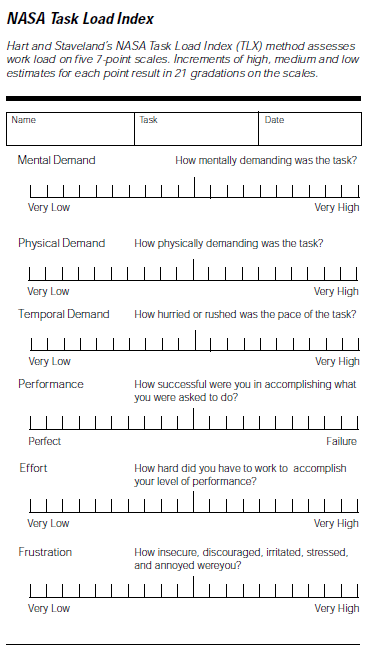
\includegraphics[width=0.7\linewidth]{figures/NasaTLX}
	\caption[پرسش نامه‌ی شاخص بار کاری ناسا]{نمونه‌ی معیار پرسش‌نامه‌ی شاخص بار کاری ناسا}
	\label{fig:nasatlx}
\end{figure}

اخيرا در یک بازتاب از استفاده از این شاخص، هارت متوجه شد كه این مقياس عمدتا در مطالعه‌هایی كه 
بر روی طراحی واسط  و  ارزیابیها متمركز  بودند، استفاده  شده  است  كه  شامل  تأثير خودكارسازی و 
تصميمگيری بودند.
\cite{hart2006nasa}
\\
علاوه بر این، مطابق با اهداف اصلی كه برای آن طراحی شده، در بسياری از مطالعه‌ها كنترل ترافيک
هوایی و سایر فعاليتهای هوافضایی استفاده شده است. در مقابل، پژوهشگران نظریهی بار شناختی كه 
روی محيط یادگيری متمركز شده بودند و از این مقياس استفاده كردند، اغلب ساختار آن را با انتخاب 
بعضی زیرمقياسها تغيير دادند .همچنين صورت برخی از سوالها را نيز عوض كردند.
\cite{antonenko2010using}
در تلاش برای
اندازه‌گيری دسته‌های مختلف بار شناختی، شایتر، گرجتز ،و كاتامبن سه مورد از سوال‌ها را انتخاب كردند:
«نيازمندی‌های كار( »
\LTRfootnote{Task demands}
مقدار فعاليت ذهنی و فيزیکی برای انجام تکليف یادگيری نياز بود؟) ،«تلاش» (به 
چه ميزان تلاش و كار نياز بود تا دانش آموز مفاهيم درس را متوجه شود؟) و «نيازمندیهای هدایت»
\LTRfootnote{Navigation demands}
)شركت كننده باید به چه ميزان تلاش كند تا محيط آموزش را كنترل كند؟). گرجتز و همکاران استدلال 
كردند كه هركدام از این موارد می‌تواند به ترتيب ،متناظر با بار شناختی ذاتی، وابسته و فرعی باشد. نتایجی
از یک مطالعه كه پيچيدگی مثال‌های كار شده را دستكاری می‌كرد نشان داد كه موافقت گسترده‌ای با 
داده‌های عملکرد وجود دارد. به عبارت دیگر، گروه‌هایی با بالاترین ميزان یادگيری، كمترین ميزان بار 
شناختی را گزارش كردند. با این حال، شواهدی برای مشاركت این سه معيار با انواع مختلف بار شناختی
ذكرشده ،وجود ندارد.
\cite{gerjets2006can}
\\
\paragraph{اصل حجم‌کاری ورودی ترافیک هوایی}
این اصل که به اختصار 
ATWIT
\LTRfootnote{Air Traffic Workload Input Technique}
خوانده می‌شود، اولین بار توسط استین معرفی شد.
\cite{stein1985air}
این معیار در مقایسه با معیار ناسا که تنها می‌تواند در انتهای فعالیت شناختی استفاده شود، آزدی بیشتری دارد و این اجازه را می‌دهد تا در حین فرآیند یادگیری از آن استفاده شود. این معیار برای سیستم‌ها و مطالعه‌های کنترل ترافیک هوایی طراحی شده با این حال در حوزه های دیگر نیز مورد بررسی قرار گرفته و عملکرد آن ثابت شده است. در این روش از یک مقیاس ۱( حجم‌کاری کم) تا ۷ (حجم کاری زیاد) نمره‌ای استفاده می‌شود که در این حین فرآیند یادگیری کاملا متوقف شده و از یادگیرنده خواسته می‌شود تا بار کاری خود را گزارش کند. یکی از مزیت های استفاده از این روش آن است که به ما اجازه می‌دهد تا ارزیابی دقیق تری در حین آزمایش شناختی داشته باشیم، به جای آنکه تا انتهای آزمایش صبر کنیم و بار شناختی را گزارش دهیم. در تصویر
\ref{fig:atwit}
نمونه‌ای از این پرسشنامه را می‌بینید.

\begin{figure}[htbp]
	\centering
	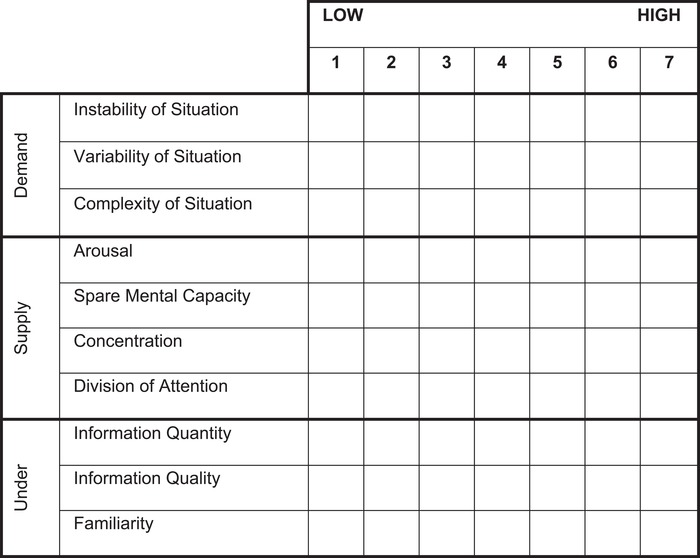
\includegraphics[width=0.7\linewidth]{figures/ATWIT}
	\caption[پرسش نامه‌ی ترافیک‌هوایی]{در پرسشنامه حجم‌کاری ترافیک هوایی مقیاس ها از ۱ تا ۷ هستند. و می‌توان در طول فرآیند آزمایش از یادگیرنده گرفته شود.}
	\label{fig:atwit}
\end{figure}

در جستجوی معيارهای متفاوت‌تری برای بار شناختی، تمایل به اصلاح جمله‌های پرسش‌نامه به نحوی كه
با  انواع مختلف  بار  شناختی متناظر  باشند، به  وجود  آمد.  برای برخی از  پژوهشگران  از  مواردی مانند
«محتوای آموزشی برای شما چقدر دشوار بود؟ چقدر برایتان مشکل بود تا مفاهيم را یاد بگيرید؟ چقدر در 
طول یادگيری تمركز داشتهاید؟» استفاده كردند. دليل این جمله بندی برقراری ارتباط با سه سطح مختلف 
بار شناختی بود. سؤال اول مربوط به بار ذاتی، سؤال دوم مربوط به بار فرعی و سؤال سوم نيز در رابطه با بار 
وابسته است. در این مطالعه، بين اندازهگيریهای شناختی بار و دادههای كارآیی، ارتباط قابل توجهی
یافت شد. با این حال، گاهی وقت‌ها  ارتباط‌های بين آزمون  كارآیی و  اندازه‌گيری‌های بار  شناختی با 
پيشبينی‌های نظری تطابق ندارد. در تعدادی از مطالعه‌ها جمله بندی‌های با تنوع بيشتری را به كار بر دند. 
از دانش آموزان خواسته شد تا به «دشواری دامنه» (بار ذاتی) و «چقدر تلاش برای درک مفاهيم مثالها 
انجام  دادید؟» (بار وابسته) امتيازدهی كنند.  با این حال، این مطالعه  ارتباط  مورد  انتظار  بين
اندازهگيریهای بار شناختی و نتایج یادگيری را نيافت.
\cite{sweller2011measuring}
\\
ناسازگاریهای فوق در تلاشهای روانسنجی برای اندازهگيری انواع مختلف بار شناختی غيرمنتظره
نيست. تمایزهای روانشناسانه بين دستههای مختلف بار شناختی نياز به این دارد كه یادگيرندگان نشان 
دهند كه به چه ميزان از هر دستهی بار شناختی متحمل شدند. ما به یادگيرندگان شک داریم، به خصوص 
یادگيرندگان تازه وارد قادر به ایجاد تمایز موردنياز نيستند.
\cite{sweller2011measuring}
\\